% บทนี้จะถูกเปลี่ยนเป็น "ภาคผนวก ก, ข, ..." อัตโนมัติเมื่อรันผ่านไฟล์หลัก
\chapter{ที่เก็บซอร์สโค้ดและขั้นตอนการติดตั้งเพื่อใช้งานระบบ}

\section{ที่เก็บซอร์สโค้ดของโครงงาน}
โครงงานนี้ได้แบ่งการพัฒนาออกเป็น 2 ส่วนหลัก ได้แก่ ส่วนของเว็บแอปพลิเคชัน สำหรับจัดการข้อมูล และส่วนของอุปกรณ์ไอโอที สำหรับตรวจจับอุณหภูมิ โดยสามารถเข้าถึงซอร์สโค้ดได้ดังนี้:

\begin{itemize}
    \item \textbf{Web Application (Frontend/Backend):} \\
    \url{https://github.com/bambiiisadeer/TempTrack.git}
    \item \textbf{IoT Devices (Microcontroller \& Sensors):} \\
    \url{https://github.com/phuennae/TempTrack_IoTs.git}
\end{itemize}

\section{ขั้นตอนการติดตั้งเพื่อใช้งานระบบ}
ในการติดตั้งและเตรียมความพร้อมของระบบโครงงานบน Cloud Server (AWS EC2 - Ubuntu) ได้แบ่งขั้นตอนการติดตั้งตามองค์ประกอบหลักของระบบออกเป็น 5 ส่วน ดังนี้

\subsection{การติดตั้งและรันระบบเว็บแอปพลิเคชัน}
% --- พื้นที่เว้นไว้ให้ผู้เขียนเติมรายละเอียดการรัน Web App (รอข้อมูลจากเพื่อน) ---
(อยู่ระหว่างการรวบรวมรายละเอียดขั้นตอนการตั้งค่าและรัน Web Application)

\vspace{2em}

\subsection{การติดตั้งและตั้งค่า MQTT Broker บน AWS EC2}
ในการรับส่งข้อมูลอุณหภูมิจากอุปกรณ์ IoT ไปยังเซิร์ฟเวอร์ โครงงานนี้ใช้โปรโตคอล MQTT โดยทำการติดตั้ง Mosquitto Broker บนเซิร์ฟเวอร์ตามขั้นตอนดังนี้:

\begin{verbatim}
# 1. อัปเดตแพ็กเกจของระบบ
sudo apt-get update

# 2. ติดตั้ง Mosquitto Broker และ Client
sudo apt-get install mosquitto mosquitto-clients -y

# 3. ตั้งค่าให้ Mosquitto ทำงานอัตโนมัติเมื่อเปิดเซิร์ฟเวอร์
sudo systemctl enable mosquitto
sudo systemctl start mosquitto
\end{verbatim}
\textit{*หมายเหตุ: จำเป็นต้องเปิดพอร์ต 1883 ในหน้า Security Group ของ AWS EC2 เพื่อรับข้อมูลจากภายนอก}

\vspace{2em}

\subsection{การติดตั้งและตั้งค่าเครือข่าย Hyperledger Fabric บน AWS EC2}
การรันเครือข่ายบล็อกเชนจำเป็นต้องติดตั้ง Docker และเครื่องมือสภาพแวดล้อมพื้นฐาน ดังนี้:

\begin{verbatim}
# 1. ติดตั้งเครื่องมือพื้นฐานและ Docker
sudo apt-get install curl git jq docker.io docker-compose -y
sudo usermod -aG docker $USER

# 2. ดาวน์โหลดสคริปต์และติดตั้งไบนารีของ Hyperledger Fabric
curl -sSLO https://raw.githubusercontent.com/hyperledger/fabric/main/scripts/install-fabric.sh
chmod +x install-fabric.sh
./install-fabric.sh docker samples binary
\end{verbatim}

\vspace{2em}

\subsection{การเตรียมอุปกรณ์ไอโอทีและการอัปโหลดโค้ด}
ก่อนเริ่มการส่งข้อมูลเข้าสู่ระบบ จำเป็นต้องอัปโหลดโค้ดลงสู่บอร์ดไมโครคอนโทรลเลอร์ โดยต้องตั้งค่าตัวแปรเพื่อให้บอร์ดเชื่อมต่อกับเซิร์ฟเวอร์ได้ถูกต้อง ดังนี้:

\begin{itemize}
    \item \textbf{WiFi Configuration:} แก้ไขค่า \texttt{ssid} และ \texttt{password} ในซอร์สโค้ดให้ตรงกับ WiFi ในพื้นที่ติดตั้ง
    \item \textbf{Server Configuration:} แก้ไขหมายเลข IP Address (Public IP) ของ AWS EC2 Server ในโค้ดส่วนของ MQTT Broker ให้ถูกต้อง
    \item \textbf{Code Uploading:} ใช้โปรแกรม Arduino IDE ในการเบิร์นโค้ด (Burn) ลงสู่บอร์ดเพื่อให้บอร์ดเริ่มทำงานและส่งข้อมูลอุณหภูมิ
\end{itemize}

\vspace{2em}

\subsection{การรันเซอร์วิสเชื่อมต่อข้อมูล IoT เข้าสู่บล็อกเชน}
เมื่อเตรียมระบบพื้นฐานและอุปกรณ์ IoT เรียบร้อยแล้ว ให้รันสคริปต์ตัวกลาง (Bridge) เพื่อดึงข้อมูลจาก MQTT เข้าสู่บล็อกเชน ดังนี้:

\begin{verbatim}
# 1. ติดตั้งไลบรารีที่จำเป็นสำหรับ Node.js
npm install

# 2. รันสคริปต์หลักเพื่อเริ่มกระบวนการรับและบันทึกข้อมูล
node server.js
\end{verbatim}

หากการตั้งค่าในหัวข้อก่อนหน้าถูกต้อง ระบบจะแสดงผลลัพธ์การรับข้อมูล (Recv) และสถานะการบันทึกสำเร็จ (Saved to Blockchain) ดังรูปที่ \ref{fig:backend_terminal}

\begin{figure}[H]
    \centering
    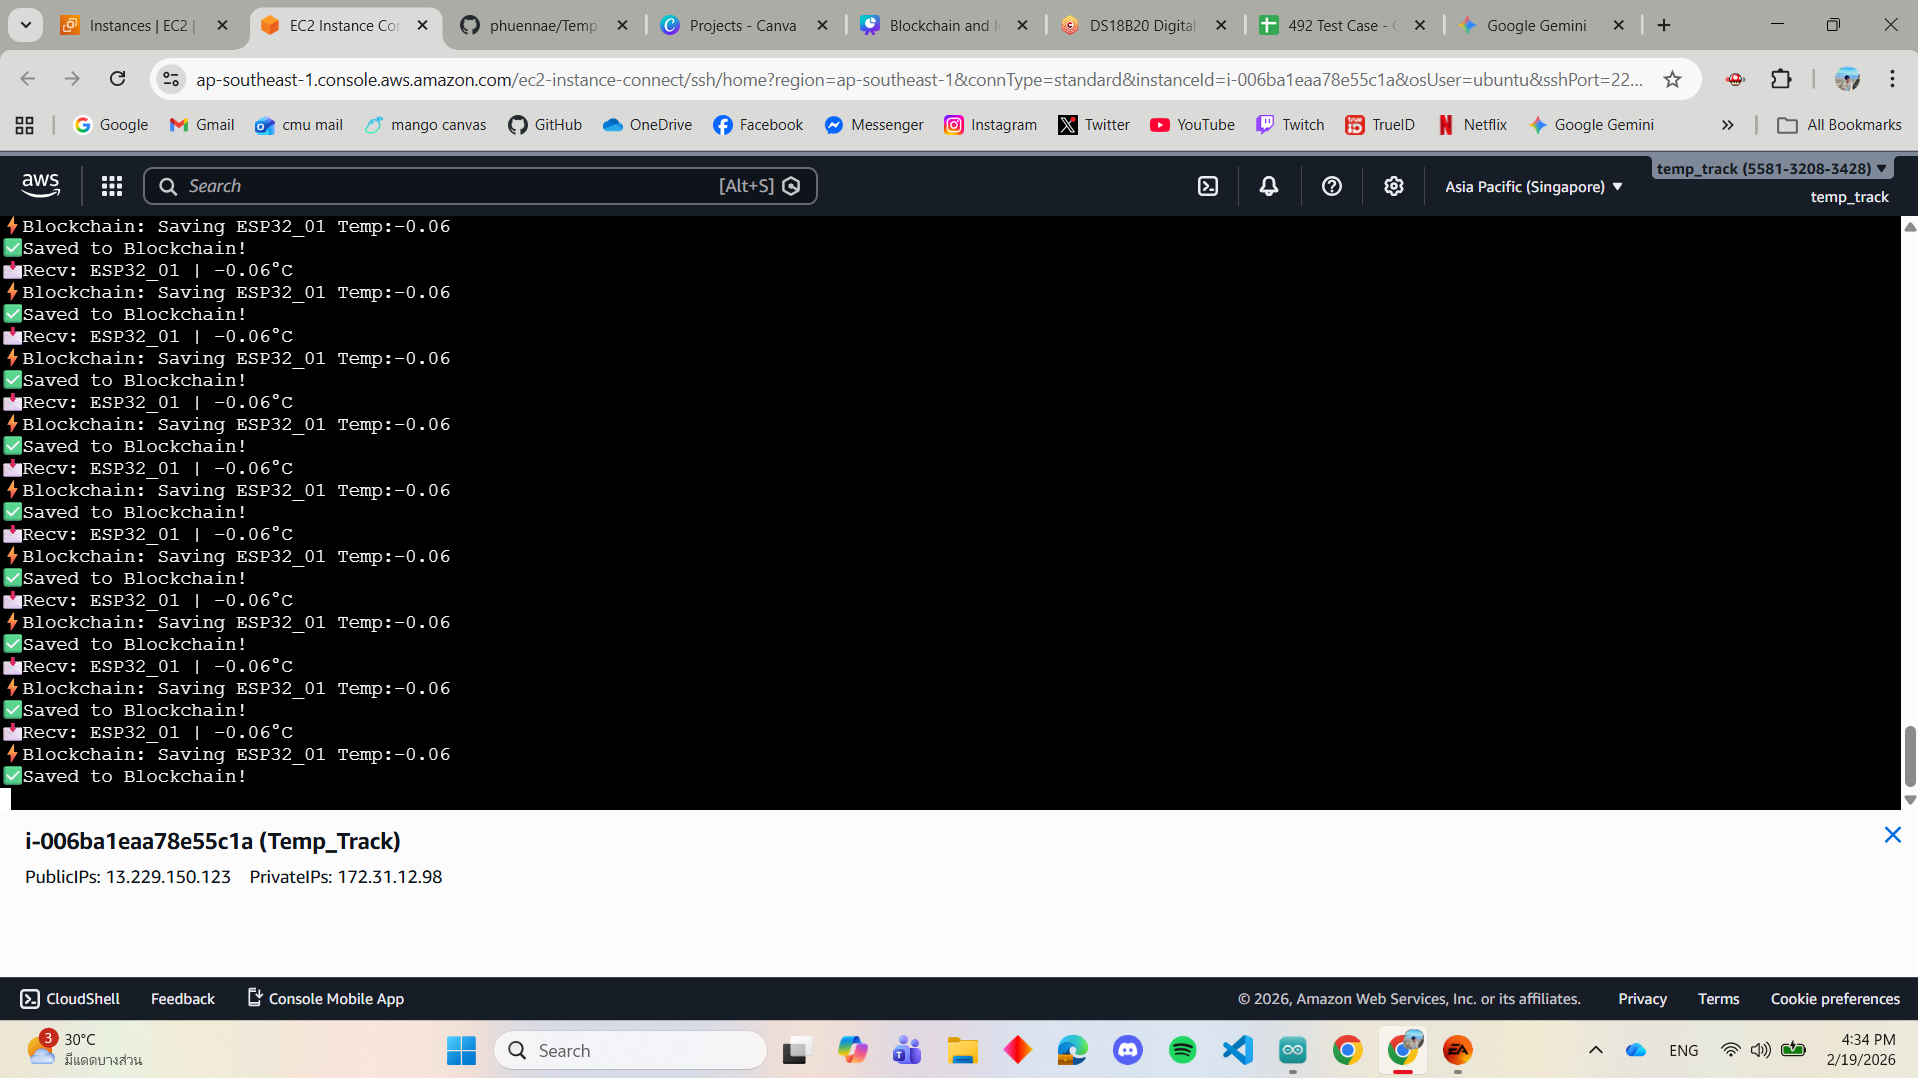
\includegraphics[width=0.85\textwidth]{AWS EC2 Server Terminal.png} 
    \caption{หน้าจอแสดงผลการทำงานขณะระบบรับข้อมูลและบันทึกลงบล็อกเชนสำเร็จ}
    \label{fig:backend_terminal}
\end{figure}


\chapter{รายละเอียดฮาร์ดแวร์และการต่อวงจร}

\section{การต่อวงจรเซ็นเซอร์อุณหภูมิและบอร์ดควบคุม}
ในส่วนนี้แสดงแผนผังการต่อสายระหว่างบอร์ดไมโครคอนโทรลเลอร์กับเซ็นเซอร์วัดอุณหภูมิ DS18B20

\begin{figure}[H]
     \centering
     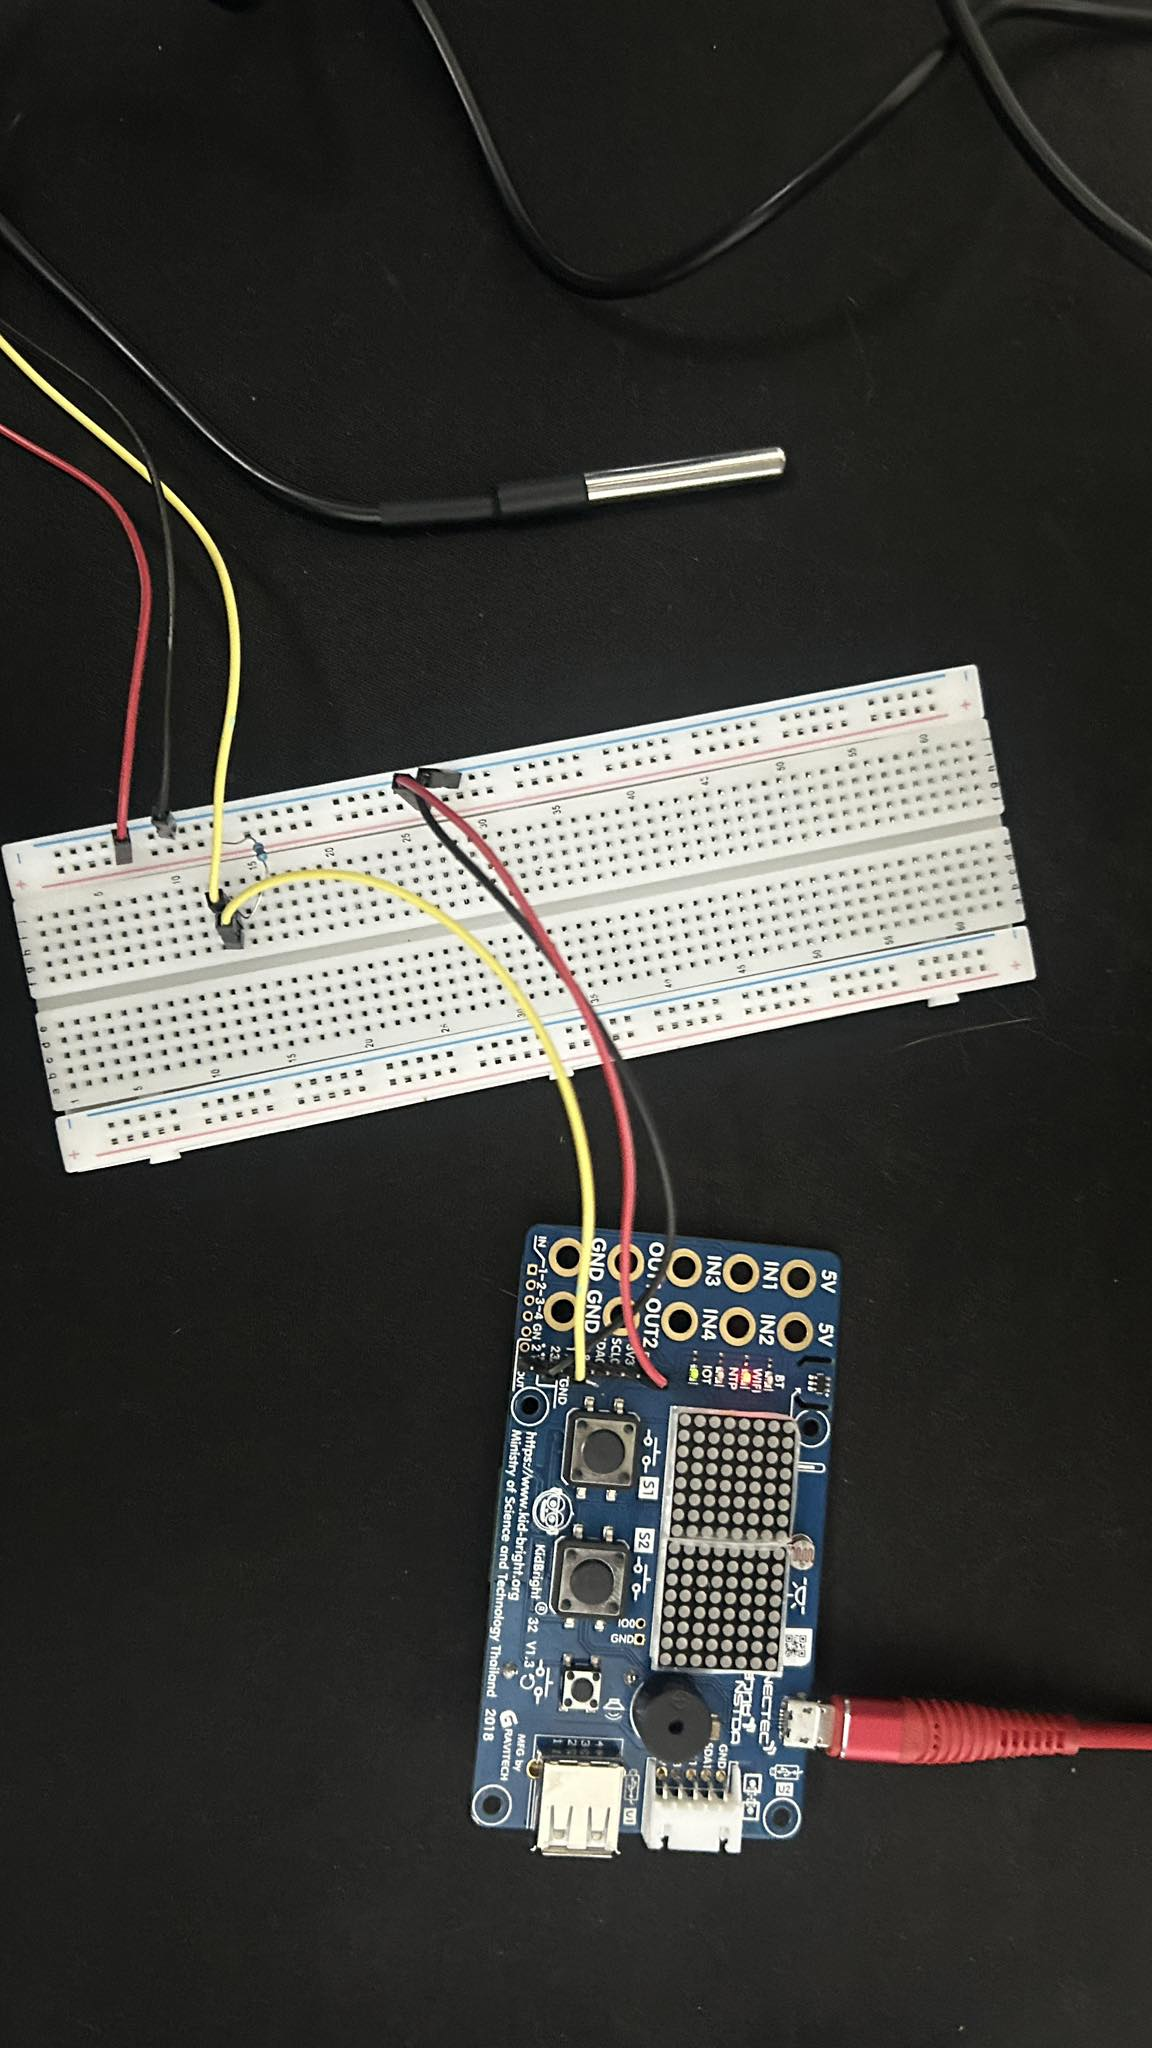
\includegraphics[angle=-90, width=0.9\textwidth]{492 wiring diagram.jpg}
     \caption{แผนผังการต่อวงจรฮาร์ดแวร์ของโปรเจกต์ TempTrack}
 \end{figure}


\chapter{โครงสร้างซอร์สโค้ด}

\section{โครงสร้างซอร์สโค้ดฝั่ง IoT}
หน้าที่ของไฟล์หลักในฝั่ง IoT มีรายละเอียดดังนี้:
\begin{itemize}
    \item[] \textbf{\texttt{DS18B20\_example.ino}} : โค้ดทดสอบการอ่านค่าอุณหภูมิเบื้องต้น
    \item[] \textbf{\texttt{Temptrack\_MQTT.ino}} : โค้ดหลักที่ใช้อ่านอุณหภูมิและส่งผ่าน MQTT
\end{itemize}

\section{ซอร์สโค้ดส่วนเชื่อมต่อข้อมูล (MQTT to Blockchain Bridge)}
ในไฟล์ \texttt{server.js} มีลอจิกสำคัญในการดักฟังข้อมูลและสั่งบันทึกลงบล็อกเชน พร้อมทั้งแสดงสถานะการทำงาน (Log) ออกทางหน้าจอ ดังนี้:

\begin{verbatim}
client.on('message', async (topic, message) => {
    const data = JSON.parse(message.toString());
    console.log(`Recv: ${data.sensor_id} | ${data.temp}`);

    try {
        await contract.submitTransaction('CreateRecord', data.temp);
        console.log('Saved to Blockchain!');
    } catch (e) {
        console.log('Error: ', e);
    }
});
\end{verbatim}

\section{โครงสร้างซอร์สโค้ดฝั่ง Web Application}
(อยู่ระหว่างการรวบรวมรายละเอียดโครงสร้างไฟล์ฝั่ง Web Application)

\newpage